\chapter{System Model}
\label{cha:system}
\vspace{0.4 cm}

In this chapter, the model of the proposed system is presented.
In the first section, an in-depth presentation of the system architecture is provided.
The different components of the system with their functionalities and the interactions among them are described.
Lastly, the three modules focused on the three use cases of interest are treated more in detail in dedicated sections.
After this chapter, it will be clear what the main parts of the system are and how they cooperate to accomplish the various use cases of interest.


\section{System architecture}
\label{sec:architecture}
\vspace{0.2 cm}

The system architecture of the developed system is shown in figure~\ref{fig:components}.
It contains the following components:
\begin{itemize}
  \item Authentication layer: manages authentication and permissions of users;
  \item API layer: manages the user interactions with the system;
  \item Task manager: coordinates the execution of the tasks;
  \item Data storage task: parses and stores the loaded data;
  \item ML model interface: handle interactions with the ML models storage where the trained models are stored;
  \item Training task: trains new models based on available data;
  \item Forecasting task: forecasts new data using a specified model or the latest model;
  \item Task scheduler: manages periodic scheduled tasks;
  \item Performance evaluation task: evaluates the performance of the available models and if needed triggers the re-training.
\end{itemize}

The system interacts with the following external components:
\begin{itemize}
  \item Users DB: used for storing and retrieving user data (possibly more users for the same account);
  \item Data DB: used for storing and retrieving the data;
  \item ML models storage: used for storing and retrieving the trained models;
  \item Forecasts DB: used for storing and retrieving the computed forecasts.
\end{itemize}

\begin{figure}[H]
\centering 
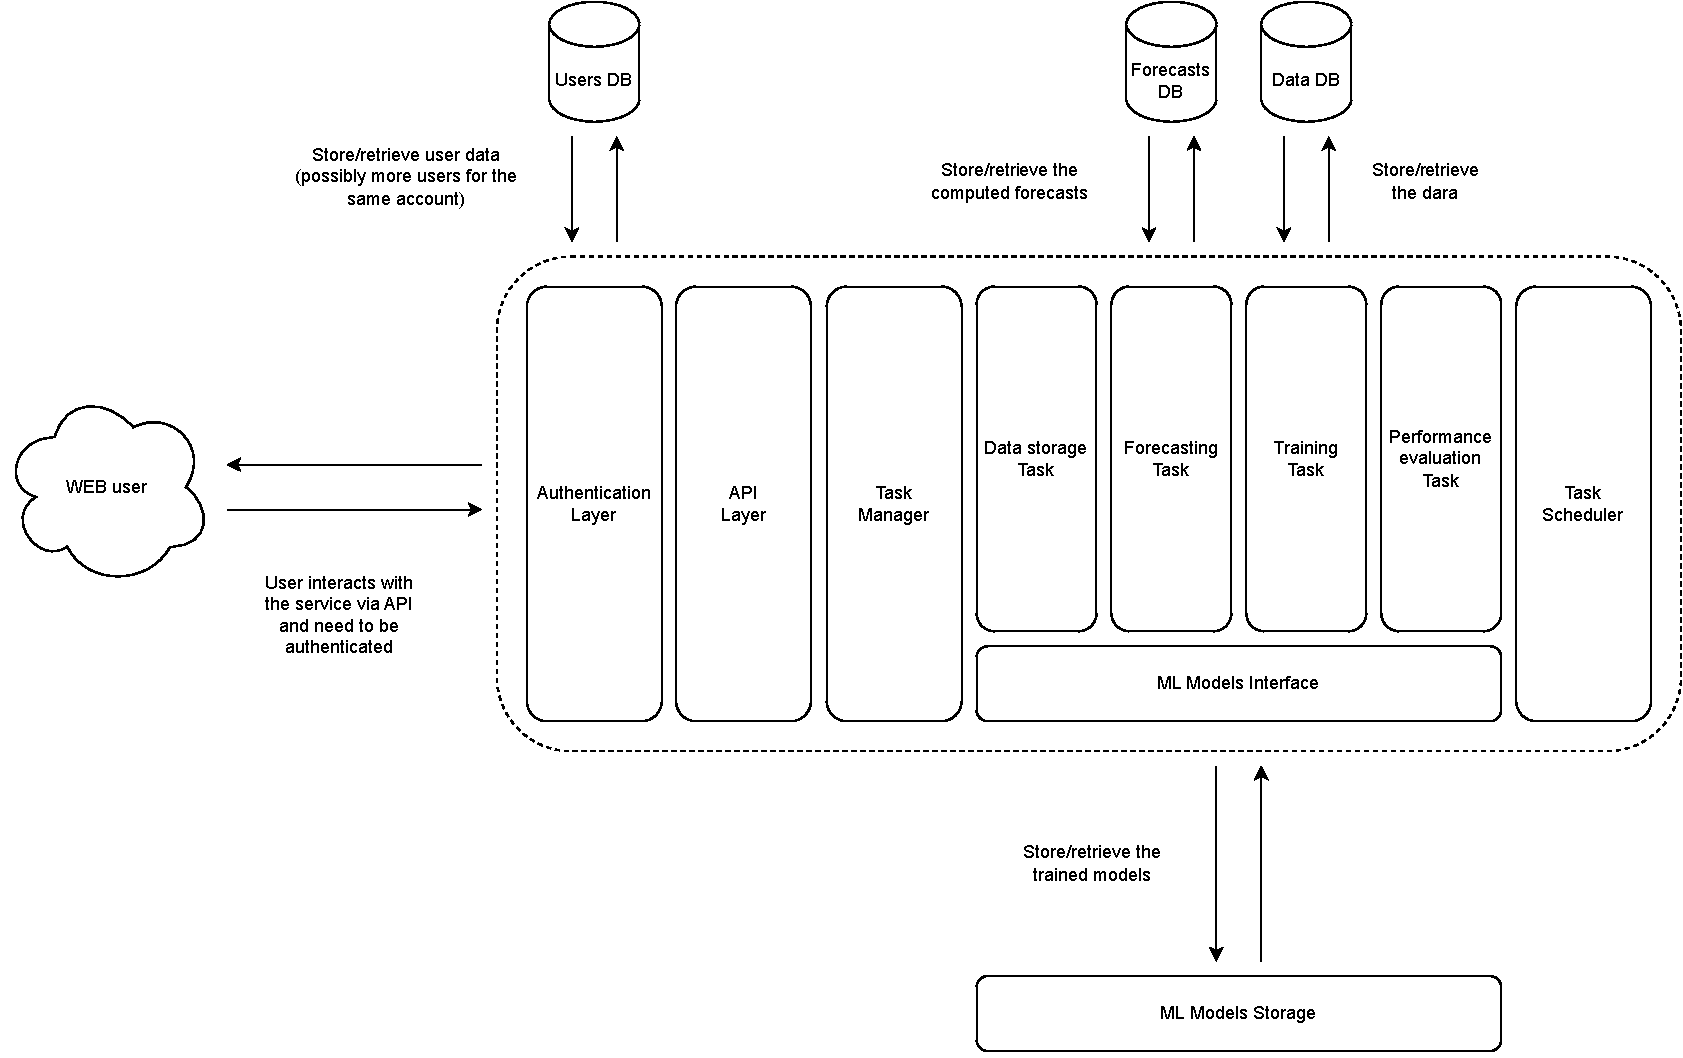
\includegraphics[width=0.9\textwidth]{images/architecture_components}
\caption{The architecture of the proposed system.}
\label{fig:components}
\end{figure}

Figure~\ref{fig:interactions} shows the interactions among the components of the architecture.

\begin{figure}[H]
\centering 
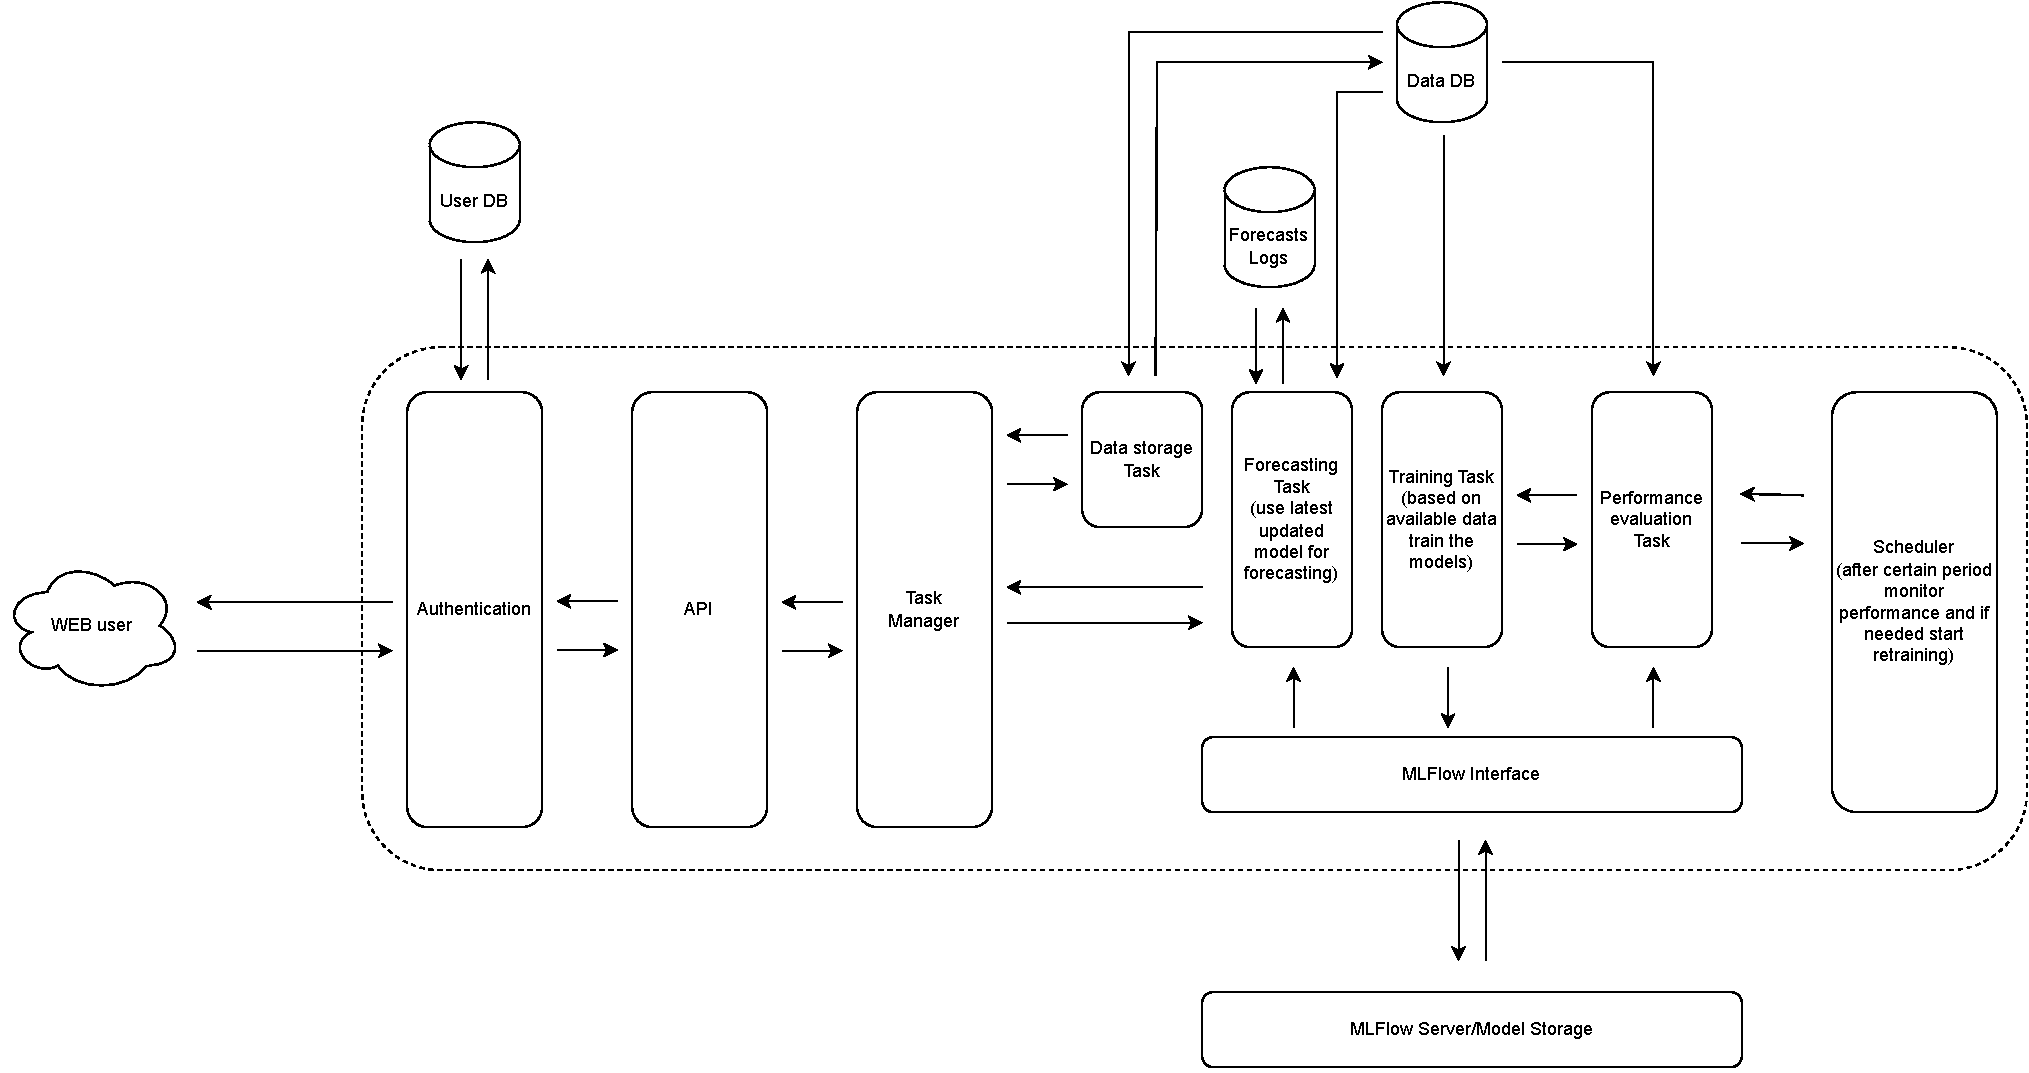
\includegraphics[width=1\textwidth]{images/architecture_interactions}
\caption{The interactions of the components of the proposed system.}
\label{fig:interactions}
\end{figure}

The use case diagram for the system is presented in figure~\ref{fig:usecase}.
Users can interact with the system via API.
A user must be authenticated and have an account with an active subscription.
Then, he can request the following asynchronous operations:
\begin{itemize}
  \item Append new data with a create or update logic specifying the type of data, it supports upload of CSV files;
  \item Train new models based on available data for a use case specifying the time granularity (hourly or daily);
  \item Forecast new data for a use case using a specified model or the latest model for a certain time granularity, for a certain starting date and time horizon.
\end{itemize}

In addition, the task scheduler periodically triggers the performance evaluation task for evaluating the performance of the available models and if needed triggering the re-training for having up-to-date models with respect to the user data that might perform better on future forecasts.

\begin{figure}[H]
\centering 
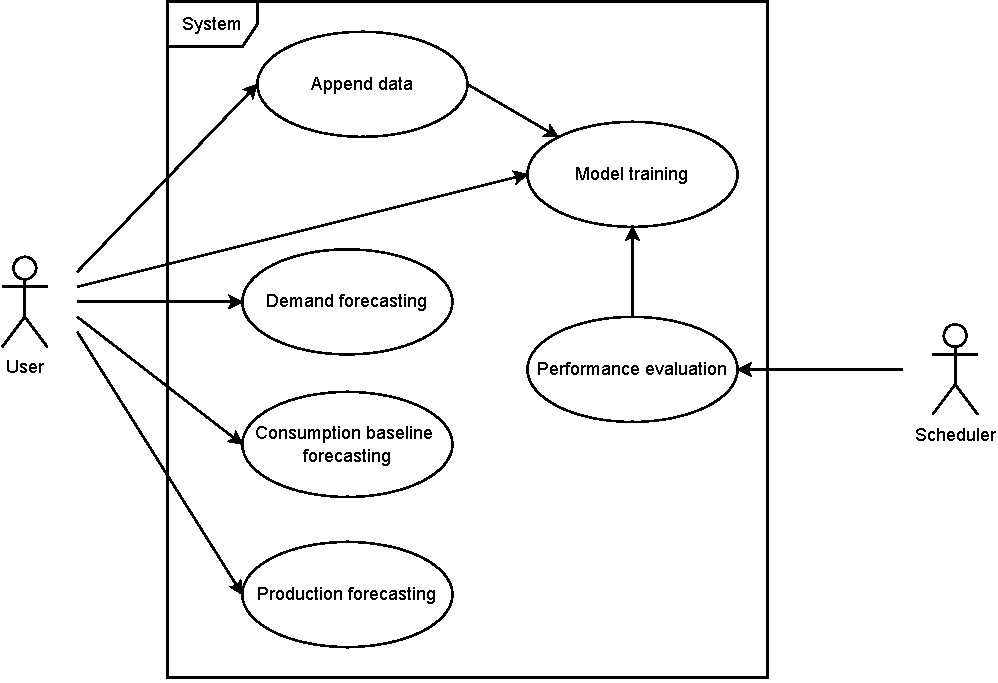
\includegraphics[width=0.6\textwidth]{images/architecture_use_case}
\caption{The use case diagram for the system.}
\label{fig:usecase}
\end{figure}

In the following diagrams, the logic inside these functionalities is described.
The diagram representing the data loading flow is presented in figure~\ref{fig:loadingflow}.
Describe it ...

\begin{figure}[H]
\centering 
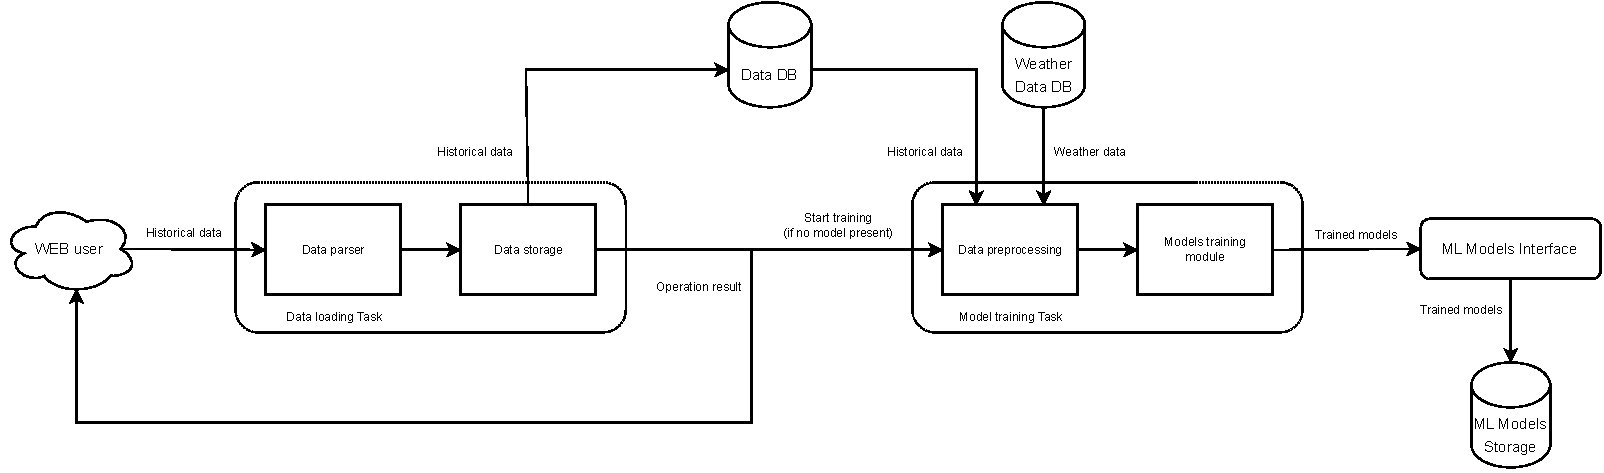
\includegraphics[width=1\textwidth]{images/architecture_data_loading_flow}
\caption{Diagram representing the data loading flow.}
\label{fig:loadingflow}
\end{figure}

The diagram representing the training flow is presented in figure~\ref{fig:trainingflow}.
Describe it ...

\begin{figure}[H]
\centering 
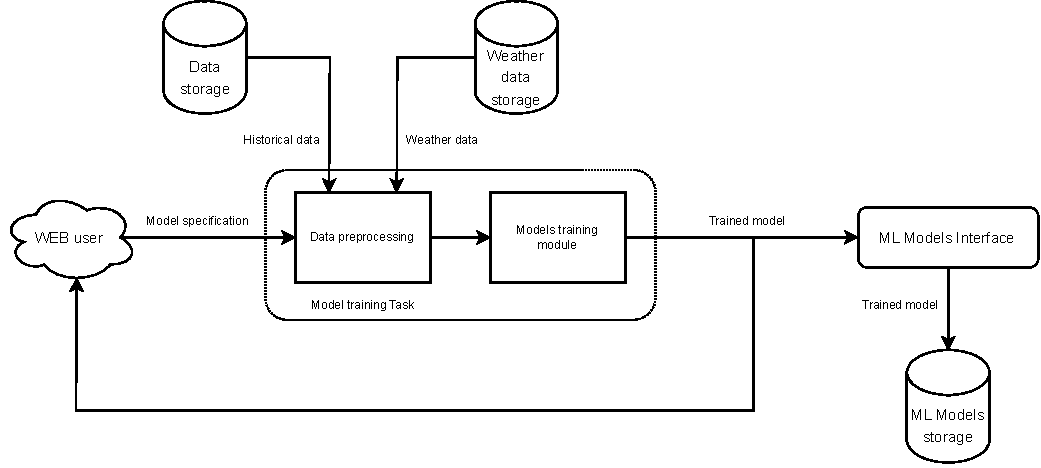
\includegraphics[width=0.7\textwidth]{images/architecture_training_flow}
\caption{Diagram representing the training flow.}
\label{fig:trainingflow}
\end{figure}

The diagram representing the forecast flow is presented in figure~\ref{fig:forecastflow}.
Describe it ...

\begin{figure}[H]
\centering 
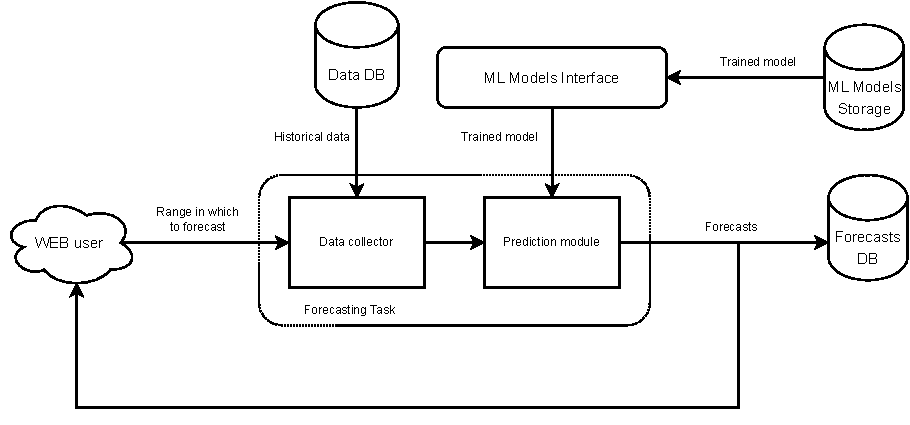
\includegraphics[width=0.6\textwidth]{images/architecture_forecast_flow}
\caption{Diagram representing the forecast flow.}
\label{fig:forecastflow}
\end{figure}

The diagram representing the task scheduler flow is presented in figure~\ref{fig:schedulerflow}.
Describe it ...

\begin{figure}[H]
\centering 
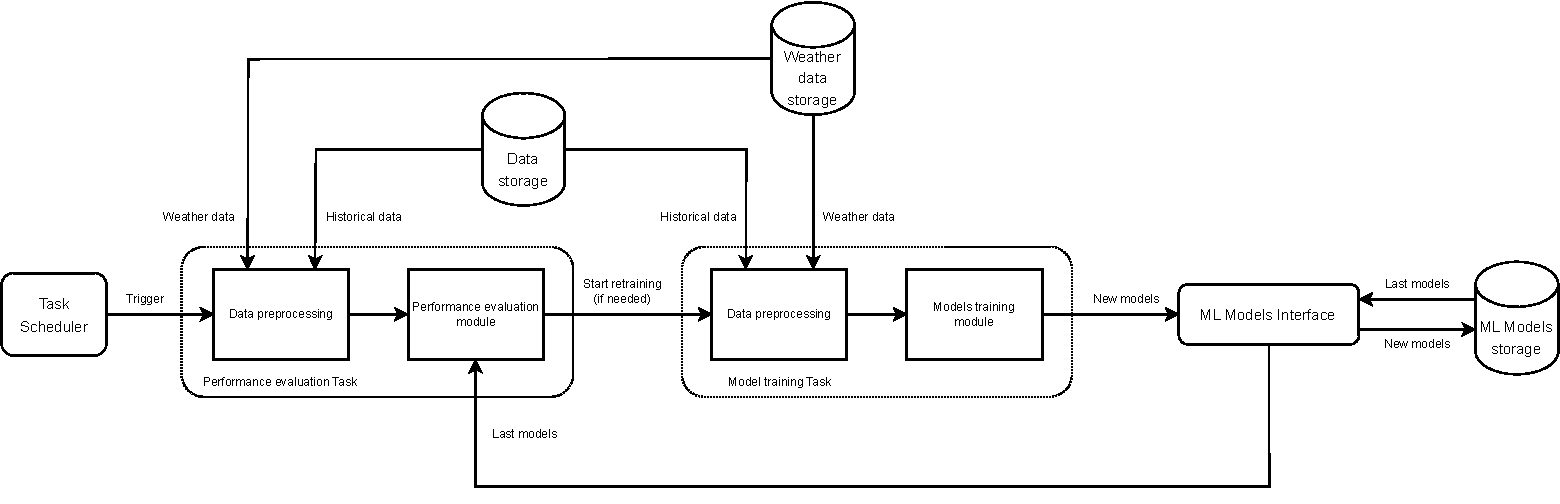
\includegraphics[width=0.8\textwidth]{images/architecture_scheduler_flow}
\caption{Diagram representing the task scheduler flow.}
\label{fig:schedulerflow}
\end{figure}

The diagram representing the data loading sequence diagram is presented in figure~\ref{fig:loadingsequence}.
Describe it ...

\begin{figure}[H]
\centering 
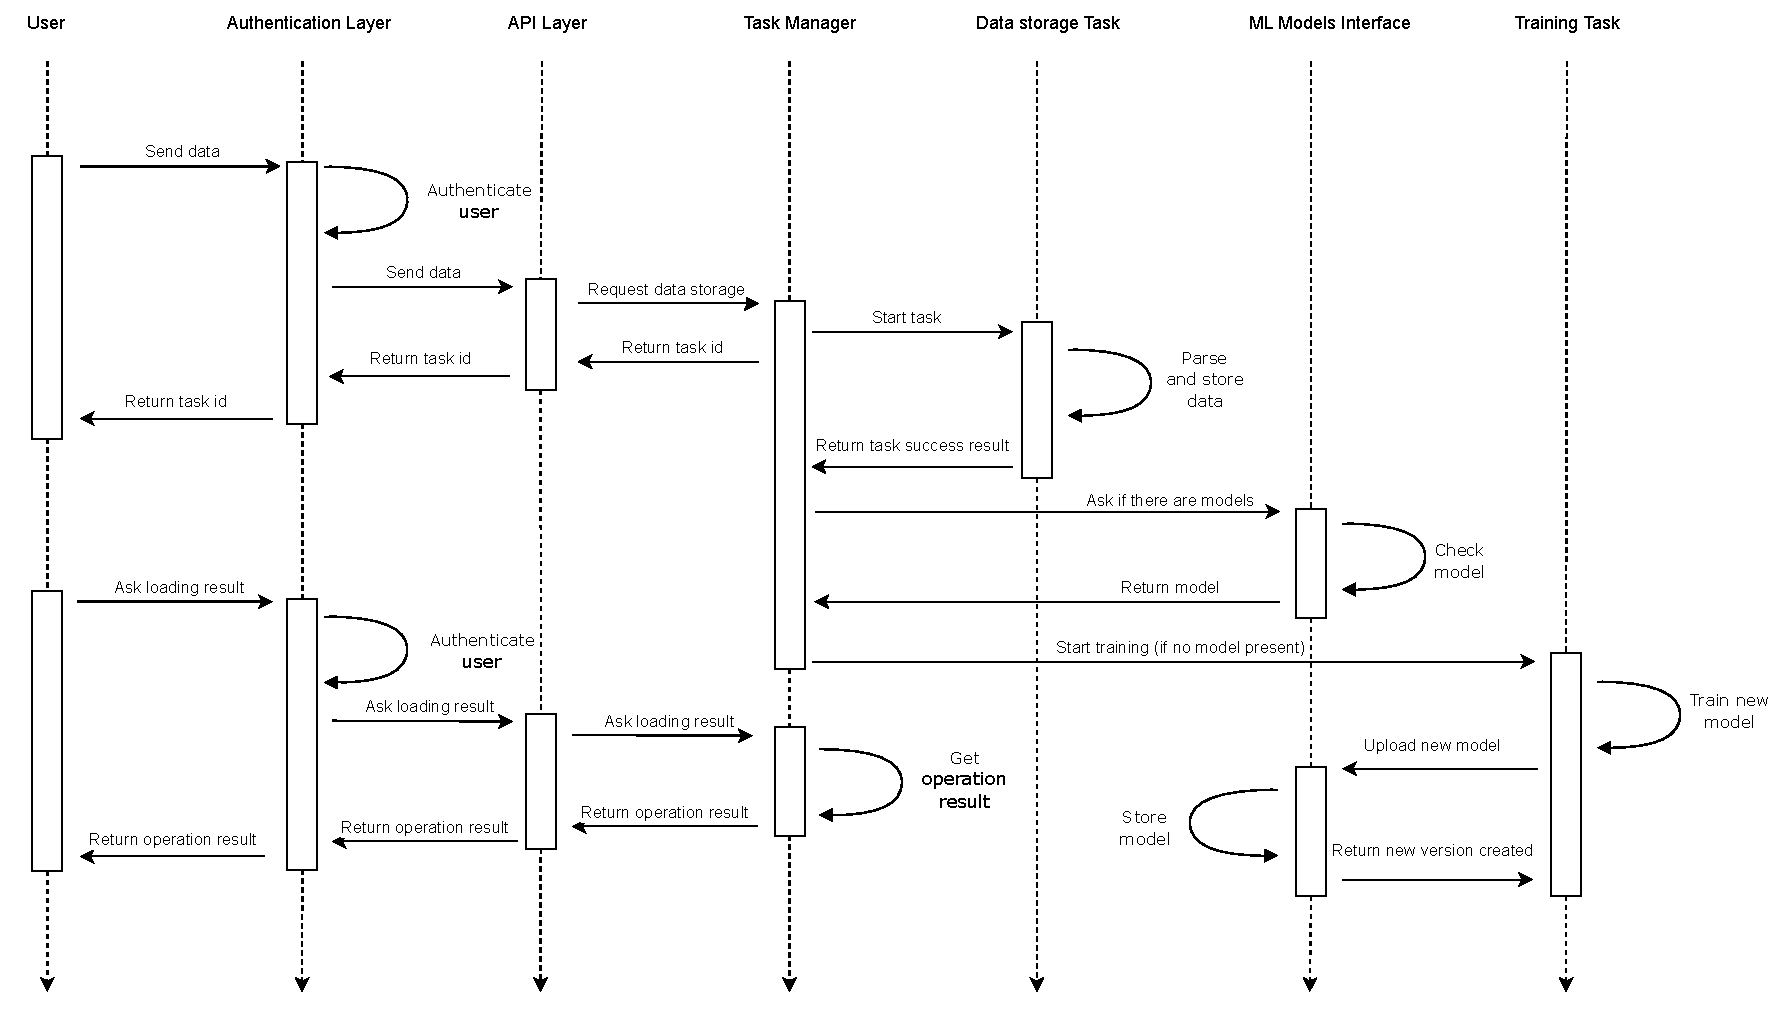
\includegraphics[width=1\textwidth]{images/architecture_data_loading_sequence}
\caption{Diagram representing the data loading sequence diagram.}
\label{fig:loadingsequence}
\end{figure}

The diagram representing the training sequence diagram is presented in figure~\ref{fig:trainingsequence}.
Describe it ...

\begin{figure}[H]
\centering 
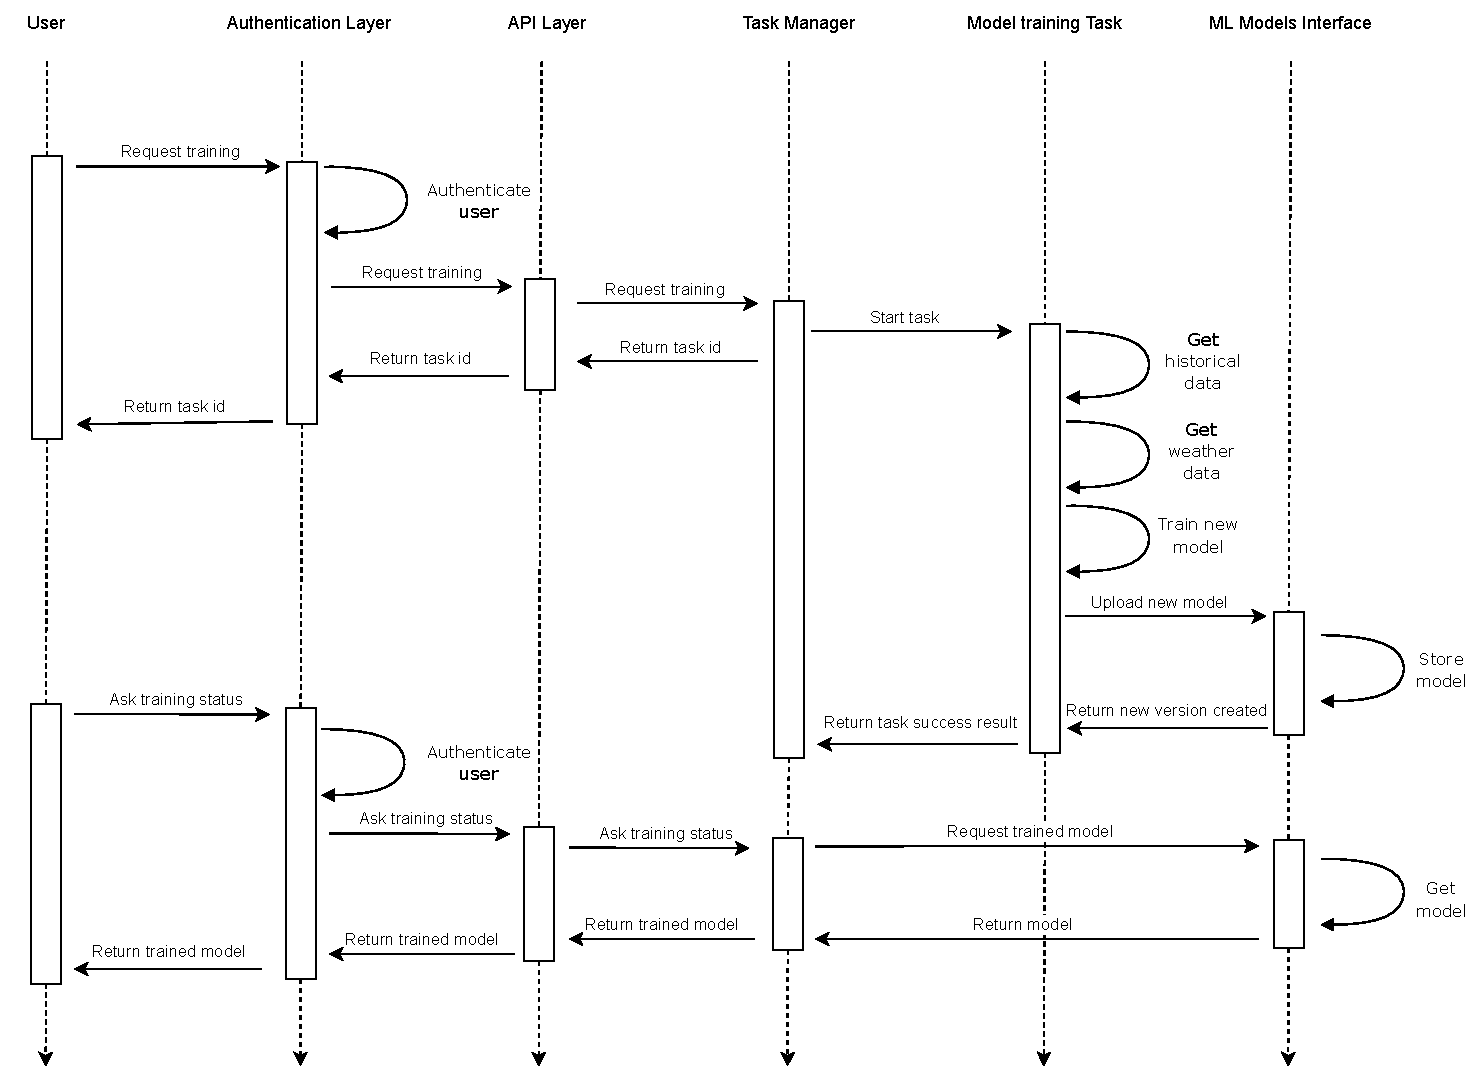
\includegraphics[width=0.8\textwidth]{images/architecture_training_sequence}
\caption{Diagram representing the training sequence diagram.}
\label{fig:trainingsequence}
\end{figure}

The diagram representing the forecasting sequence diagram is presented in figure~\ref{fig:forecastingsequence}.
Describe it ...

\begin{figure}[H]
\centering 
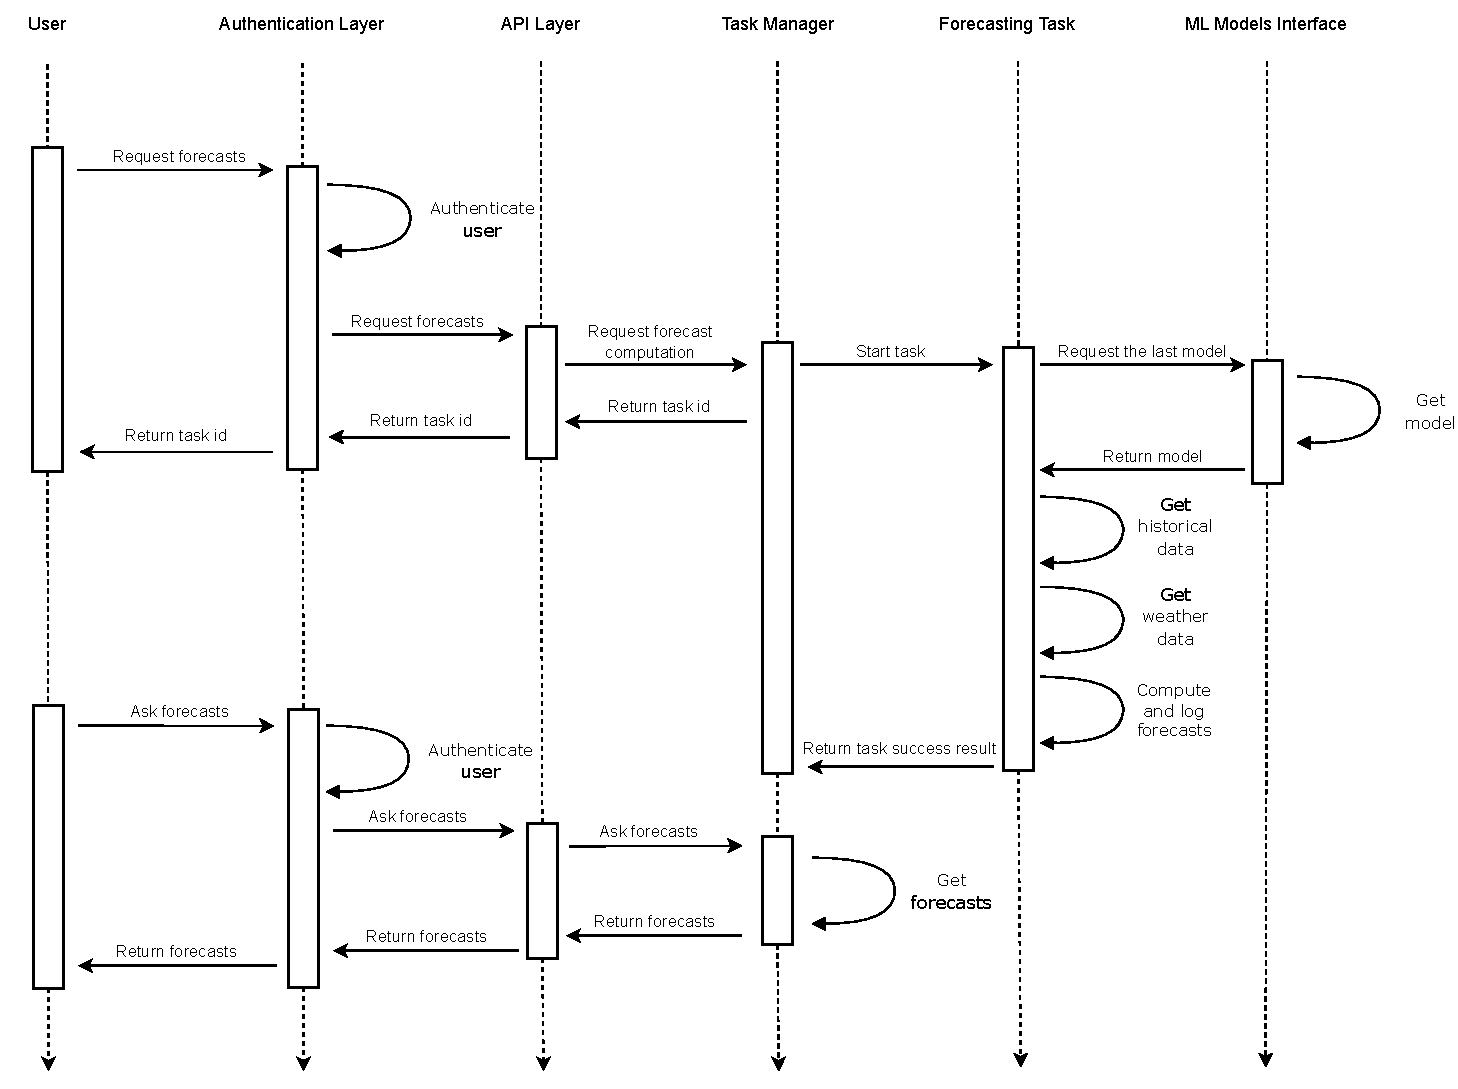
\includegraphics[width=0.8\textwidth]{images/architecture_forecasting_sequence}
\caption{Diagram representing the forecasting sequence diagram.}
\label{fig:forecastingsequence}
\end{figure}

The diagram representing the task scheduler sequence diagram is presented in figure~\ref{fig:schedulersequence}.
Describe it ...

\begin{figure}[H]
\centering 
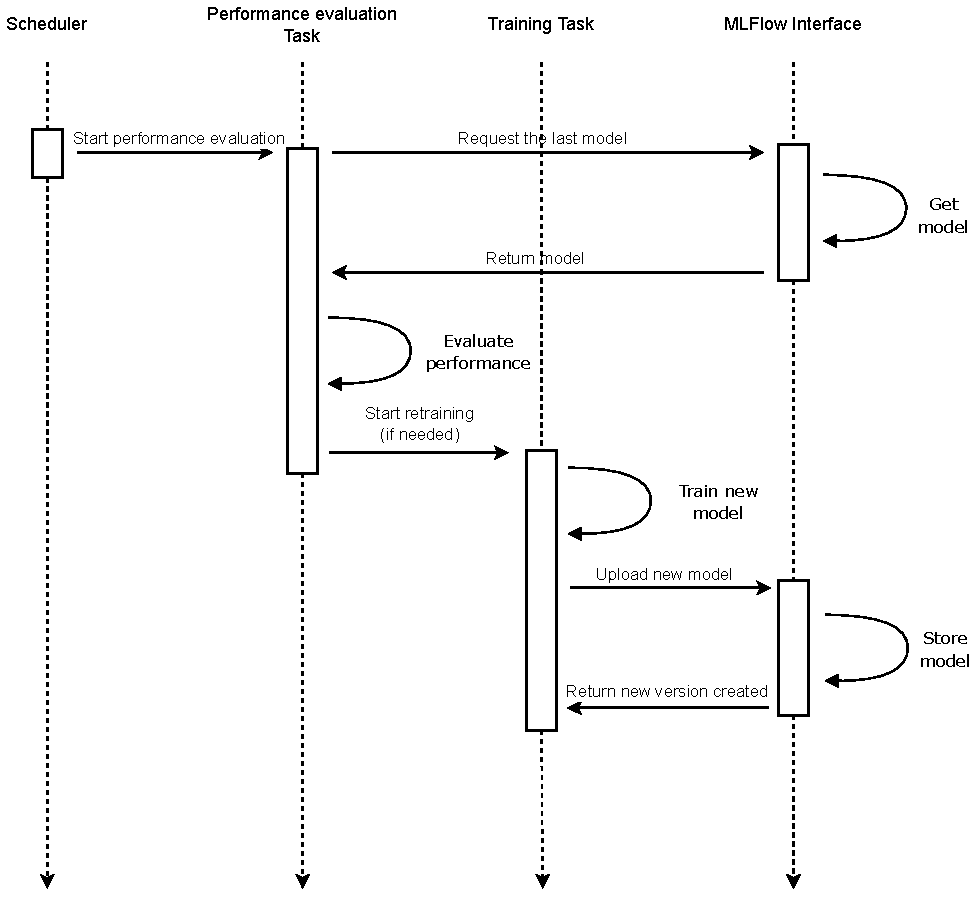
\includegraphics[width=0.6\textwidth]{images/architecture_scheduler_sequence}
\caption{Diagram representing the task scheduler sequence diagram.}
\label{fig:schedulersequence}
\end{figure}


\section{System common components}
\label{sec:components}
\vspace{0.2 cm}

Describe the system's common components between the various tasks ...

Describe Data Parser/Preprocessing, enrichment, Model Training Procedure, Prediction, ...

The system model training schematic representation is presented in figure~\ref{fig:modeltraining}.

\begin{figure}[H]
\centering 
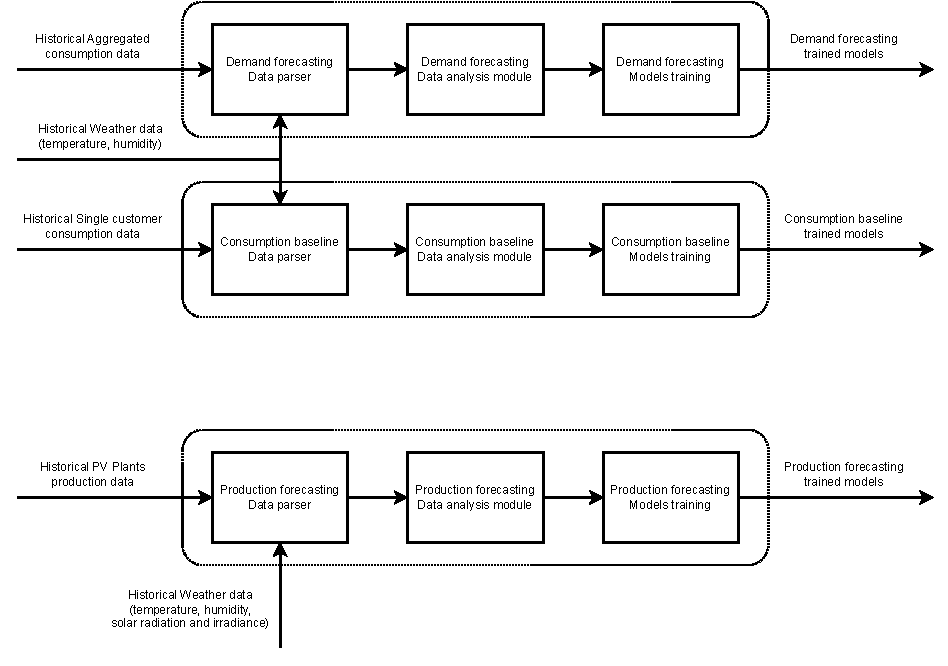
\includegraphics[width=1\textwidth]{images/system_model_training}
\caption{The system model training schematic representation.}
\label{fig:modeltraining}
\end{figure}

The system model forecasting schematic representation is presented in figure~\ref{fig:modelforecasting}.

\begin{figure}[H]
\centering 
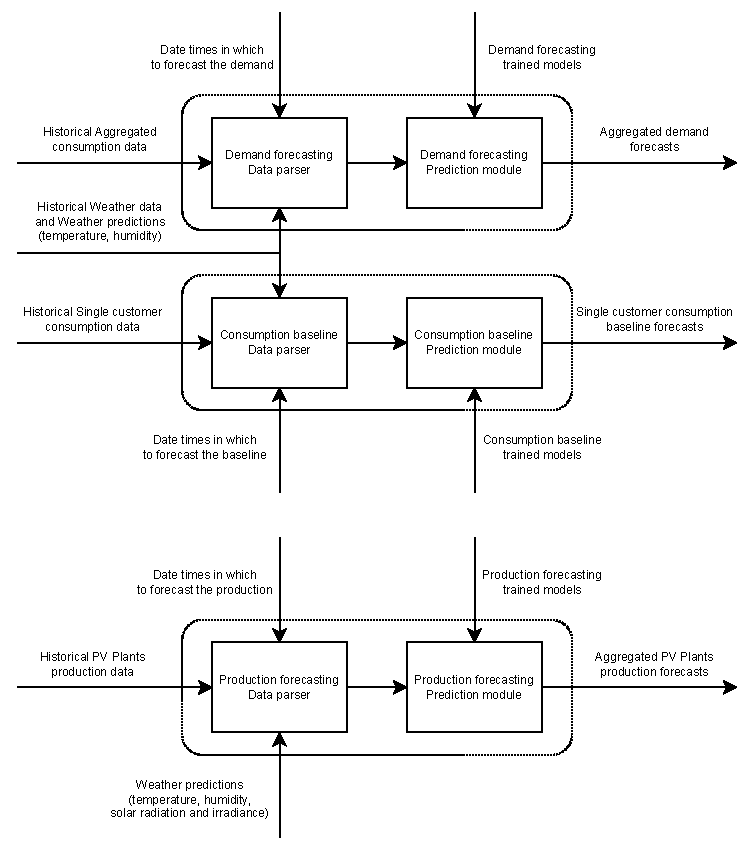
\includegraphics[width=0.8\textwidth]{images/system_model_forecasting}
\caption{The system model forecasting schematic representation.}
\label{fig:modelforecasting}
\end{figure}


\section{Electricity demand forecasting module}
\label{sec:demandmodel}
\vspace{0.2 cm}

Describe the electricity demand forecasting module ...

How the module works, what contains, Models used for the task-specific and then report also in the sections below if they are common, ...

\section{Consumption baseline forecasting module}
\label{sec:baselinemodel}
\vspace{0.2 cm}

Describe the consumption baseline forecasting module ...


\section{Electricity production forecasting module}
\label{sec:productionmodel}
\vspace{0.2 cm}

Describe the electricity production forecasting module ...
